
\chapter{Forecasting}
\label{cha:forecasting}

\section{Prophet}

\subsection{Model overview}

Prophet is a statistical model developed by engineers at Facebook, which mainly fits its models in Stan and has been open-sourced with public APIs for python and R languages\cite{fb_prophet}. It takes a regression-fitting approach to learn the time series and then forecasts by extrapolating such models and adding uncertainty in a Bayesian framework.

It uses a decomposable time series models \cite{harvey1990estimation} with three components: trend, seasonality and holidays:

\begin{equation}
	y(t) = g(t) + s(t) + h(t) + \varepsilon_t
\end{equation}

Where $g(t)$ is a trend function that models non-periodic fluctuations, $s(t)$ capture different kinds of seasonalities, and $h(t)$ represents special situations that could add irregularities to the other components and a random error term $\varepsilon$.

The model is similar to a \ac{gam}\cite{hastie1987generalized}, which allows adding more and more components as needed. The seasonalities are modelled by an exponential smoothing approach\cite{gardner1985exponential}.

\subsection{Trend model}

Prophet has two trend models: a saturating growth one, which is similar to model population growths in ecosystems \cite{hutchinson1978introduction} and a piecewise model to give the flexibility of trend changes in determined learnt changepoints \cite{fb_prophet}.

The basic saturated growth model is given by

\begin{align}\label{eq:sat_growth}
		g(t) &= \frac{C}{1 + \exp\left\{ -k(t-m) \right\}}
\end{align}

\begin{equation*}
	\text{Where} \quad
	C: \text{Carrying capacity}, \quad
	k: \text{Growth rate}, \quad
	m: \text{Offset parameter}
\end{equation*}

Nonetheless, the saturated growth model in (\ref{eq:sat_growth}) does not meet all the usual requirements for some of the applications in which the saturating ceiling varies over time or in which the growth rate is not constant. Therefore, the model has been extended as follows.

Let $s_j=1,\ldots,S$ be the number of changepoints where the growth rate is allowed to change. Then, let $\delta_j$ be the change rate that happens at $s_j$, and $\bm{\delta} \in \mathbb{R}^s$ the vector defined by all $\delta_j$. This means that the growth rate at any time $t$ is the base rate $k$ plus all the adjustments up to $t$

\begin{equation}
	k + \sum_{j=1}^{t < s_j}{\delta_j}
\end{equation}

This can be rewriten as

\begin{align}
	\begin{split}
		k &+ \bm{a}(t)^T\bm{\delta} \\
		\text{Where}\quad a_j &= 
		\begin{cases*}
			1\quad,\quad\text{if} \quad t > s_j \\
			0\quad,\quad\text{otherwise}
		\end{cases*}
	\end{split}
\end{align}

Also, when the growth rate is adjusted, the $m$ needs to be adjusted to ensure continuity. 

\begin{equation}
	\gamma_j = \left( s_j - m - \sum_{l<j}{\gamma_l} \right) \left(1 - \frac{k+\sum_{l<j}{\delta_l}}{k+\sum_{l \leq j}{\delta_l}} \right)
\end{equation}

Then the linear trend with changepoints is defined by (\ref{eq:piece_trend}) piecewise logistic growth model by (\ref{eq:piece_satgrowth})\cite{fb_prophet}.

\begin{equation}\label{eq:piece_trend}
	g(t) = \left( k + \bm{a}(t)^T \bm{\delta} \right)t + \left( m + \bm{a}(t)^T \bm{\gamma} \right)
\end{equation}

\begin{equation}\label{eq:piece_satgrowth}
	g(t) = \frac{C(t)}
	        {1 + \exp\left\{-(k+\bm{a}(t)^T\bm{\delta})(t-(m+\bm{a}(t)^T \bm{\gamma}))\right\}
	        }
\end{equation}


\subsection{Trend forecast}


After the model has learnt from a history of $T$ time points with $S$ changepoints from which each point has a rate change $\delta_j \sim \text{Laplace}(0,\tau)$. 

The trend will keep its last growth rate constant. The forecasts will be made by extrapolating the \ac{gam} and simulating samples from Laplace$(0,\lambda)$ where $\lambda$ is a variance inferred from the data from the maximum likelihood estimate of the rate scale parameter (\ref{eq:lambda_inferr}).

\begin{equation}\label{eq:lambda_inferr}
	\lambda = \frac{1}{2} \sum_{j=1}^{S}{|\delta_j|}
\end{equation}

Once $\lambda$ has been inferred the trend forecast and its uncertainty are obtained from

\begin{equation}\label{eq:trend_forecast}
\forall j > T\quad,\quad 
	\begin{cases}
		\delta_j = 0 \quad \text{w.p.} \frac{T-S}{S} \\
		\delta_j \sim \text{Laplace}(0,\lambda) \quad \text{w.p.} \frac{S}{T}
	\end{cases}
\end{equation}

\pagebreak
\subsection{Seasonalities}

By using the \ac{gam} flexibility, it is possible to add different seasonality periods, 365.25 or 7 for yearly and weekly seasonalities -in days measurements-, for example. These seasonalities are modelled by the use of Fourier series\cite{harvey_fourier}.

Therefore, for every given period $P$, it can be defined that.

\begin{equation}
	s(t) = \sum_{n=1}^{N}\left( a_n \cos\left( \frac{2 \pi n t}{P}\right)  + b_n \sin\left( \frac{2 \pi n t}{P}\right) \right)
\end{equation}

Which has $2N$ params to learn:

\begin{equation*}
	\bm{\beta} = \left[ a_1, b_1, a_2, b_2, \ldots, a_N, b_N\right]^T
\end{equation*}

In order to make the structures more manageable, it is defined a matrix of seasonalities comprised of the seasonal vectors for each time step.

\begin{equation}
	\bm{X}(t) = \left[ \cos\left( \frac{2 \pi (1) t}{P}\right), \sin\left( \frac{2 \pi (1) t}{P}\right), \dots , \cos\left( \frac{2 \pi (N) t}{P}\right), \sin\left( \frac{2 \pi (N) t}{P}\right)  \right]
\end{equation}

Thus, the seasonal component is expressed then as.

\begin{align}
	s(t) &= \bm{X}(t) \bm{\beta} \\
	\text{Where} \quad \beta &\sim \mathcal{N}(0, \sigma^2)
\end{align}


\subsection{Holidays and festivities}

Prophet also allows considering non-seasonal events that can significantly affect the forecasts due to changes in peoples behaviour. Namely, Muslim Ramadan, Chinese New Year or the US's Super Bowl.

It is assumed that each holiday is independent. For each holiday $i$, $D_i$ is the set of past and future dates of it. 

Same as seasonalities, a regressors matrix is generated indicating whether the time $t$ happens during holiday $i$ and a parameter $\kappa_i$ to model its influence in the forecast.

\begin{align}
	Z(t) &=  \left[   \bm{1}(t \in D_1), \ldots, \bm{1}(t \in D_L) \right] \\
	\therefore \quad h(t) &= Z(t)\bm{\kappa} \\
	\bm{\kappa} &\sim \mathcal{N}(0,\nu^2)
\end{align}

For practical cases, importing the holidays' dates can be done using the python-holidays open-source package \cite{Holidays}, for which an extract of available Swedish holidays is shown in Table \ref{table:sv_holidays}.

\begin{table}[H]
	\centering
	\begin{tabular}{|c|c|}
		\hline
		\textbf{Date} & \textbf{Holiday} \\
		\hline
		2021-01-01 &Nyårsdagen \\
		2021-01-06 &Trettondedag jul \\
		2021-04-02 &Långfredagen \\
		2021-04-04 &Påskdagen, Söndag \\
		2021-04-05 &Annandag påsk \\
		2021-05-01 &Första maj \\
		2021-05-13 &Kristi himmelsfärdsdag \\
		2021-05-23 &Pingstdagen, Söndag \\
		2021-06-06 &Sveriges nationaldag, Söndag \\
		2021-06-25 &Midsommarafton \\
		2021-06-26 &Midsommardagen \\
		2021-11-06 &Alla helgons dag \\
		2021-12-24 &Julafton \\
		2021-12-25 &Juldagen \\
		2021-12-26 &Annandag jul, Söndag \\
		2021-12-31 &Nyårsafton \\
		\hline
	\end{tabular}
	\caption{Results for Swedish holidays in 2021 from \texttt{python-holidays}}
	\label{table:sv_holidays}
\end{table}

It is possible also to include other parameters to extend the holiday to the neighbouring days. For more details, the reader can further investigate in \cite{fb_prophet}.

\subsection{Model fitting}

The seasonality and holiday components are then merged in a matrix $\bm{X}$ and the changepoints $\bm{a}(t)$, in a matrix $\bm{A}$. Then the model is expressed using Stan\cite{carpenter2017stan} as is shown in figure \ref{alg:stan}.

\begin{figure}[H]
\begin{lstlisting}
// Priors
k ~ normal(0, 5);
m ~ normal(0, 5);
epsilon ~ normal(0, 0.5);
delta ~ double_exponential(0, tau);
beta ~ normal(0, sigma);

// Logistic likelihood
y ~ normal(C ./ (1 + exp(-(k + A * delta) .* (t - (m + A * gamma)))) + X * beta, epsilon);

// Linear likelihood
y ~ normal((k + A * delta) .* t + (m + A * gamma) + X * beta, sigma);
\end{lstlisting}
\caption{Prophet Stan model.}
\label{alg:stan}
\end{figure}

Where \texttt{tau} and \texttt{sigma} are used to control the regularization levels.

Another handy feature that allows using \acp{gam} is to plot each component on its own, which allows the analyst to spot abnormalities when debugging a model. These plots will be shown and explained in the following sections.

\pagebreak
\subsection{Experiments}

The average \ac{psu} load signal shown in Figure \ref{fig:forecast_experiment_signal} has been chosen to run the following experiments. It is not a particularly easy signal since it contains some severe outliers in the first days that turned the power to almost zero, and at the end, the average power consumption seems to decrease.

It is necessary to notice that in every forecasting model, the longer the prediction horizon is, the more uncertainty and thus the lower performance. For this experiment, it has been decided to leave the last 10\% of data for testing purposes.

\begin{figure}[H]
	\centering
	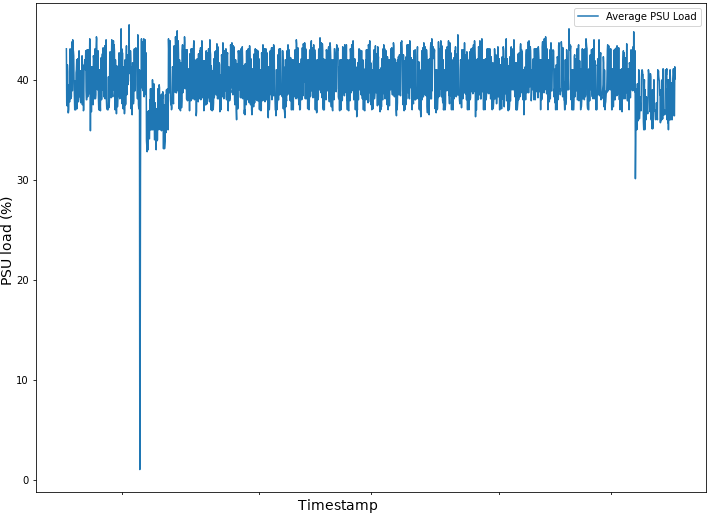
\includegraphics[width=0.6\linewidth]{forecast_experiment_signal}
	\caption{Signal used for the forecasting experiments}
	\label{fig:forecast_experiment_signal}
\end{figure}

In the following sections it is going to be shown first a pure univariate approach and later it will be added more exogenous regressors to improve the predictions. The models will be evaluated by using the following scores.

\subsubsection*{Coefficient of determination}

The coefficient of determination $R^2$ is a measure of how many variance of $\hat{y}$ is explained by the variance in $y$ in a linear regression context. It is compared against the considered \emph{worst possible linear approximation} which corresponds to the samples mean.

It is said that $R^2$ has values $[0,1]$, where $0$ corresponds to the worst linear model and 1 a perfect approximation. 

Althought the current application is not a linear regression case, $R^2$ is still considered a valuable score to compare predictor performances, nonetheless, as the linearity assumption is not met, its values would reside in $(-\infty, 1]$ where 0 still being the mean value, but it is no longer considered the worst possible fit.

\begin{equation}\label{eq:rsq}
R^2 = 1 - \frac{\sum_{i}{(y_i - \hat{y}_i)^2}}{\sum_{i}{(y_i - \bar{y}_i)^2}}
\end{equation}


\subsubsection*{Mean absolute error}

It measures, in absolute terms, the deviations from the true values. \ac{mae} is preferred, given its interpretability, over \ac{rmse} \cite{MAE}.

\begin{equation}\label{eq:mae}
\text{MAE}	= \frac{1}{N} \sum_{i=1}^{N}{ \left| y_i - \hat{y}_i \right| }
\end{equation}


\subsubsection*{Mean out-of-bounds error}

As result of the fitting process, prophet's output is comprised by the mean prediction $\hat{y}_t$ and also its lower and upper boundaries for a given confidence value when constructing the predictor object which defaults at $80\%$ 

Let then the \ac{obe} be the out-of-the-confidence-bands error defined by (\ref{eq:obe}) where $\Delta \hat{y}_t$ is the computed confidence interval half-magnitude for the time $t$. Then the \ac{mobe} can be obtained by taking the mean of these values to obtain an overall performance score as in (\ref{eq:mobe}). 

\begin{align}
\text{OBE}_i &= \bm{\min} \Big\{ \big| y_i - (\hat{y}_i - \Delta\hat{y}_i) \big| , \big	| y_i - (\hat{y}_i + \Delta\hat{y}_i) \big| \Big\} \label{eq:obe} \\
\text{MOBE} &= \frac{1}{N} \sum_{i=1}^{N}{ \text{OBE}_i }\label{eq:mobe}
\end{align}

\subsection{Univariate model implementation}

In the figure \ref{fig:prophet_uni_split} is shown the complete results of training and testing for a univariate prophet model.

\begin{figure}[H]
	\centering
	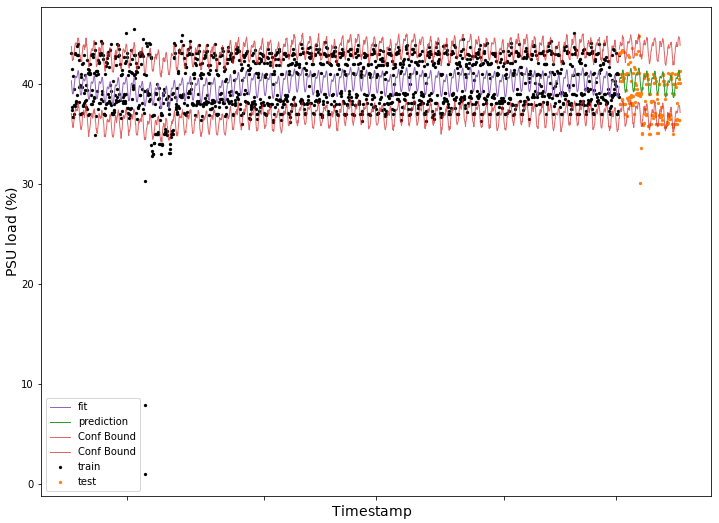
\includegraphics[width=0.6\linewidth]{prophet_uni_split}
	\caption{Training, test and predictions from univariate Prophet}
	\label{fig:prophet_uni_split}
\end{figure}

\subsubsection*{Training fitting}

In training is obtained a very poor $R^2$ value, which from the plot in figure \ref{fig:prophet_uni_fitting} can be expected, since $\hat{y}$ looks like mostly an average of the seasonal components. Nonetheless, if it is considered that predicting an interval is acceptable, then the \ac{mobe} shows a very good result. 

It can also be observed that the trend component did not overfit to the outliers.

\begin{table}[H]
	\centering
	\begin{tabular}{|c|c|}
		\hline
		\ac{mae} 	& 2.20 \\
		$R^2$ 		& 0.11 \\
		\ac{mobe} 	& 0.08 \\
		\hline
	\end{tabular}
	\caption{Univariate prophet training scores}
	\label{table:prophet_uni_train_scores}
\end{table}

\begin{figure}[H]
	\centering
	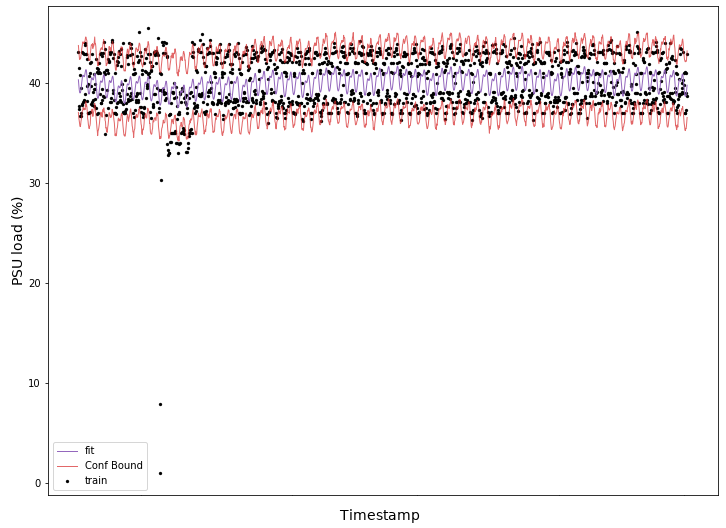
\includegraphics[width=0.6\linewidth]{prophet_uni_fitting}
	\caption{Training fitting from univariate prophet}
	\label{fig:prophet_uni_fitting}
\end{figure}

\subsubsection*{Model learnt components}

In figure \ref{fig:prophet_uni_components} it is shown the learnt approximation of every component in the \ac{gam}. Although the trend did not overfit to the outliers, still learnt that there is a break point and changed the piecewise trend.

\begin{figure}[H]
	\centering
	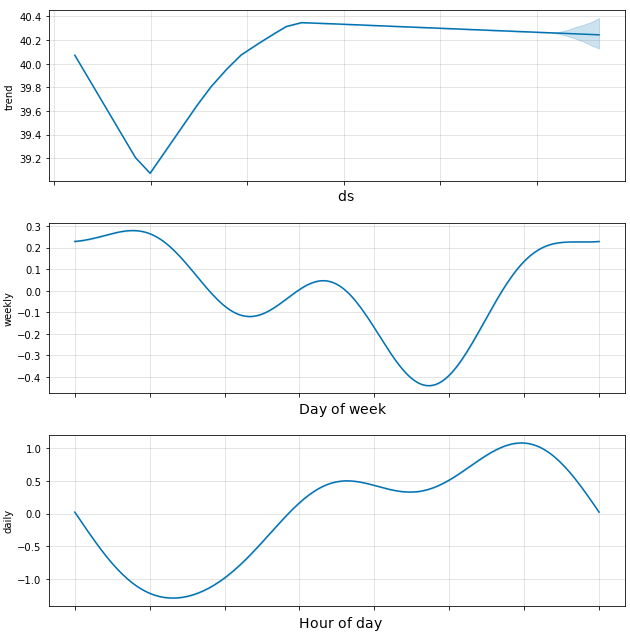
\includegraphics[width=0.7\linewidth]{prophet_uni_components}
	\caption{Learnt components from univariate prophet}
	\label{fig:prophet_uni_components}
\end{figure}

\pagebreak
\subsubsection*{Test predictions}

When it comes to the predictions performance, the $R^2$ shows even worse results. The \ac{mobe} is also high since the trend component was not able to foresee the decreasing in the middle of the test set as shown in figure \ref{fig:prophet_uni_preds}. 

\begin{figure}[H]
	\centering
	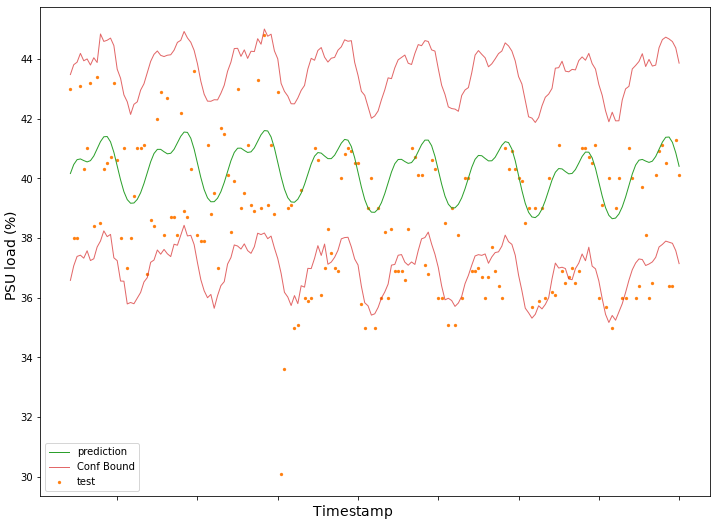
\includegraphics[width=0.6\linewidth]{prophet_uni_preds}
	\caption{Test predictions from univariate Prophet}
	\label{fig:prophet_uni_preds}
\end{figure}

\begin{table}[H]
	\centering
	\begin{tabular}{|c|c|}
		\hline
		\ac{mae} 	& 2.12 \\
		$R^2$ 		& -0.33 \\
		\ac{mobe} 	& 0.25 \\
		\hline
	\end{tabular}
	\caption{Univariate prophet prediction performance}
	\label{table:prophet_uni_test_scores}
\end{table}




\subsubsection*{Residual analysis}

The residuals in the training set still show somehow resembles the original data pattern. This could be interpreted that there is still patterns to learn from data, i.e., this model is not complete. 

\begin{figure}[hptb]
	\begin{subfigure}{.47\textwidth}
		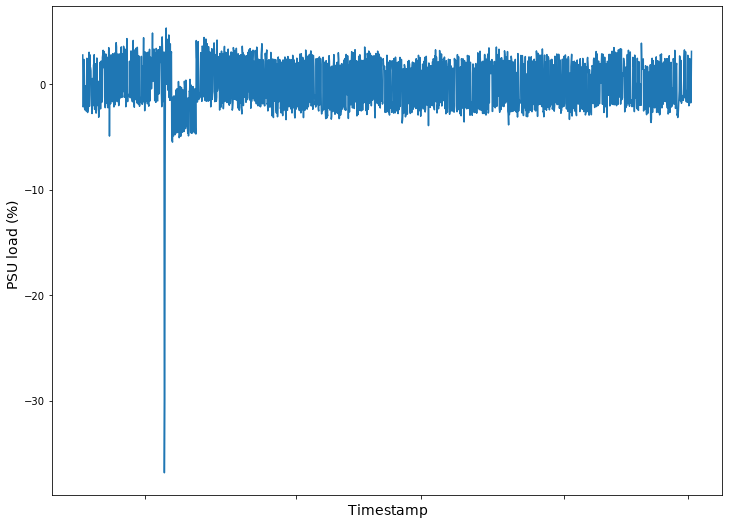
\includegraphics[width=\textwidth]{prophet_train_res_time}
		\caption{Residuals from train fit}
		\label{fig:prophet_train_res_time}
	\end{subfigure}%
	\hfill
	\begin{subfigure}{.47\textwidth}
		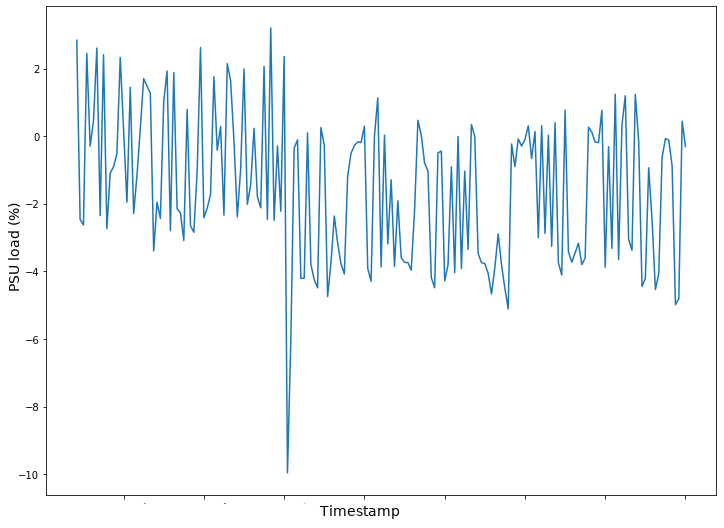
\includegraphics[width=\textwidth]{prophet_test_res_time}
		\caption{Residuals from test predictions}
		\label{fig:prophet_test_res_time}
	\end{subfigure}
	\caption{Univariate prophet residuals}
	\label{fig:prophet_res_time}
\end{figure}

Furthermore, if the joint distributions for $y$ and $\hat{y}$ are plotted, it can be seen how the outlier in the training set was not learnt and how the approximation becomes erratic in the test set.

\begin{figure}[hptb]
	\begin{subfigure}{.47\textwidth}
		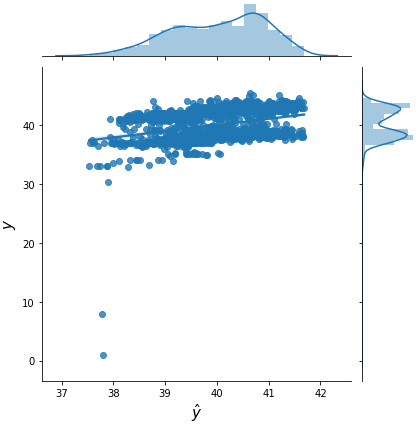
\includegraphics[width=\textwidth]{prophet_train_res_joint}
		\caption{Train}
		\label{fig:prophet_train_res_joint}
	\end{subfigure}%
	\hfill
	\begin{subfigure}{.47\textwidth}
		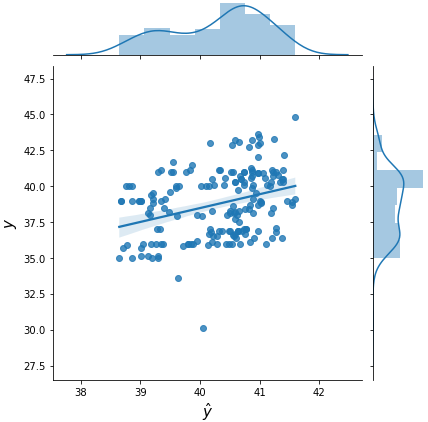
\includegraphics[width=\textwidth]{prophet_test_res_joint}
		\caption{Test}
		\label{fig:prophet_test_res_joint}
	\end{subfigure}
	\caption{Univariate prophet joint distributions of $y$ and $\hat{y}$}
	\label{fig:prophet_res_joint}
\end{figure}


\subsection{Implementation using exogenous regressors}

To fully exploit the flexibility of \acp{gam}, prophet's API allows defining custom regressors, which in the current work will be called exogenous variables as a resemblance of SARIMAX models. These variables are the ones explained in chapter \ref{cha:data_analysis}.



\subsubsection*{Model learnt components}

The model components now show the additive factor of all the exogenous regressors, which seems to contain the information not learnt by the univariate training residuals. 

\begin{table}[H]
	\centering
	\begin{tabular}{|c|c|}
		\hline
		\ac{mae} 	& 0.55 \\
		$R^2$ 		& 0.83 \\
		\ac{mobe} 	& 0.10 \\
		\hline
	\end{tabular}
	\caption{Multivariate prophet training scores}
	\label{table:prophet_multi_train_scores}
\end{table}

The $R^2$ score has considerably improved. Nonetheless, the other scores have become worse. The interpretation of this decline could be that the confidence band is now narrower than the univariate model. Thus, being out of the confidence band is now likely than before.

\begin{figure}[H]
	\centering
	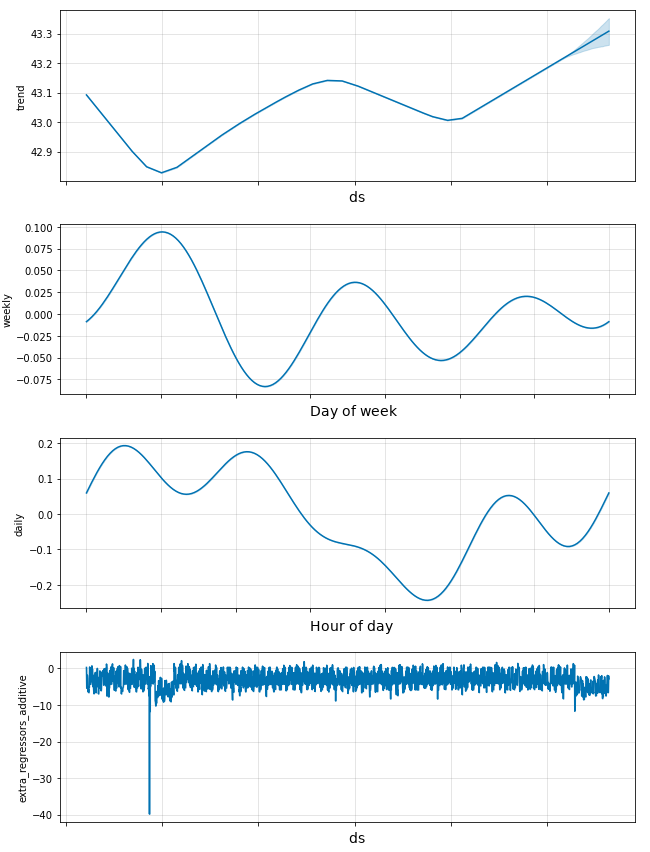
\includegraphics[width=0.7\linewidth]{prophet_multi_components}
	\caption{Learnt components from multivariate prophet}
	\label{fig:prophet_multi_components}
\end{figure}



\subsubsection*{Test predictions}

The results of the predictions have notoriously improved in this case. The $R^2$ value is close to 0.9, which for such a complex signal shows how powerful is the model. 

The \ac{mobe} has even decreased in the test set, this could be due to training outliers that still being difficult to approximate without overfitting the trend component. 

 
\begin{table}[H]
	\centering
	\begin{tabular}{|c|c|}
		\hline
		\ac{mae} 	& 0.52 \\
		$R^2$ 		& 0.88 \\
		\ac{mobe} 	& 0.05 \\
		\hline
	\end{tabular}
	\caption{Multivariate prophet prediction performance}
	\label{table:prophet_multi_test_scores}
\end{table}



\begin{figure}[H]
	\centering
	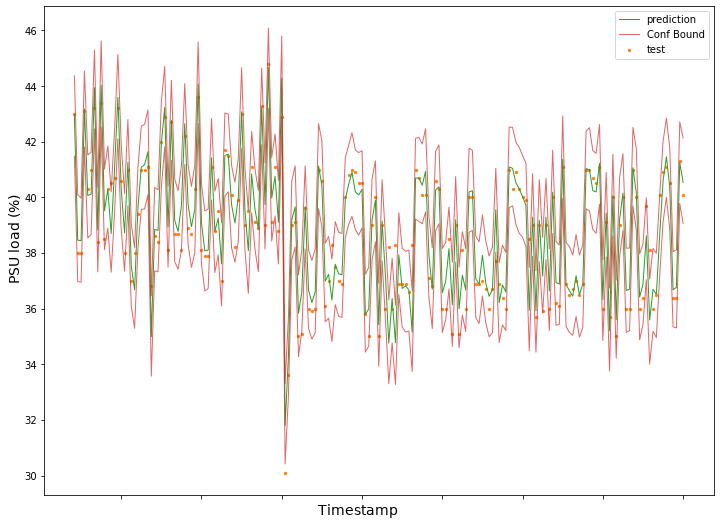
\includegraphics[width=0.6\linewidth]{prophet_multi_preds}
	\caption{Test predictions from multivariate prophet}
	\label{fig:prophet_multi_preds}
\end{figure}




\subsubsection*{Residual analysis}

The residuals now show that the patterns have been better learnt than in the univariate case.

\begin{figure}[hptb]
	\begin{subfigure}{.47\textwidth}
		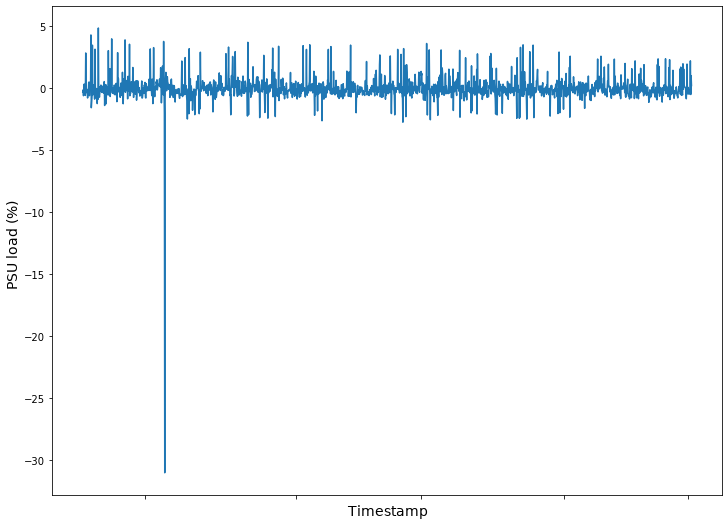
\includegraphics[width=\textwidth]{prophet_train_res_time_multi}
		\caption{Train}
		\label{fig:prophet_train_res_time_multi}
	\end{subfigure}%
	\hfill
	\begin{subfigure}{.47\textwidth}
		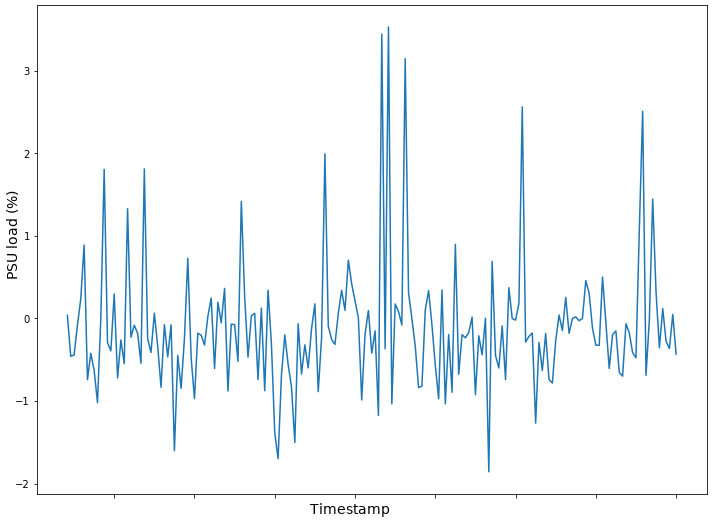
\includegraphics[width=\textwidth]{prophet_test_res_time_multi}
		\caption{Test}
		\label{fig:prophet_test_res_time_multi}
	\end{subfigure}
	\caption{Multivariate prophet residuals}
	\label{fig:prophet_res_time_multi}
\end{figure}

The joint distributions for $y$ and $\hat{y}$ now shows that the model is better approximating the signal. 

\begin{figure}[hptb]
	\begin{subfigure}{.47\textwidth}
		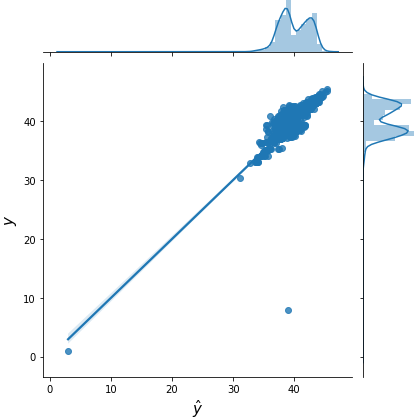
\includegraphics[width=\textwidth]{prophet_train_res_joint_multi}
		\caption{Train}
		\label{fig:prophet_train_res_joint_multi}
	\end{subfigure}%
	\hfill
	\begin{subfigure}{.47\textwidth}
		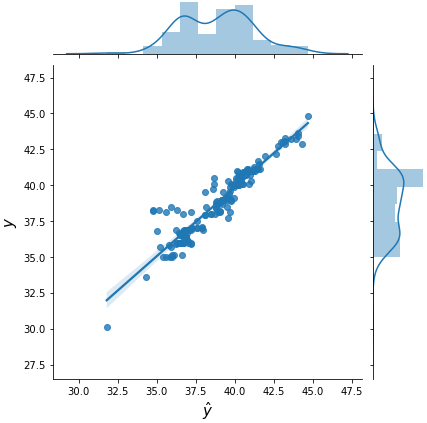
\includegraphics[width=\textwidth]{prophet_test_res_joint_multi}
		\caption{Test}
		\label{fig:prophet_test_res_joint_multi}
	\end{subfigure}
	\caption{Multivariate prophet joint distributions of $y$ and $\hat{y}$}
	\label{fig:prophet_res_joint_multi}
\end{figure}

%
%\pagebreak
%\section{Boosted random forests}
%
%
%\noindent\fbox{
%	\parbox{\textwidth}
%	{
%		Draft acknowledgement:\\
%		
%		The following models are still work in progress and last implementation has a bug to be fixed. 
%		
%		If time is not enough we may decide to drop this part for final report
%	}
%}
%
%\subsection{Model overview}
%
%\noindent\fbox{
%	\parbox{\textwidth}
%	{
%		Draft acknowledgement:\\
%		XGBoost regressor theory
%	}
%}
%
%\subsection{Regression approach}
%
%\begin{equation}
%	\label{xgb_reg}
%	y_{t+1} = \sum_{t=1}^{N}{\beta_t \cdot x_{t_i}}
%\end{equation}
%
%\begin{figure}[H]
%	\centering
%	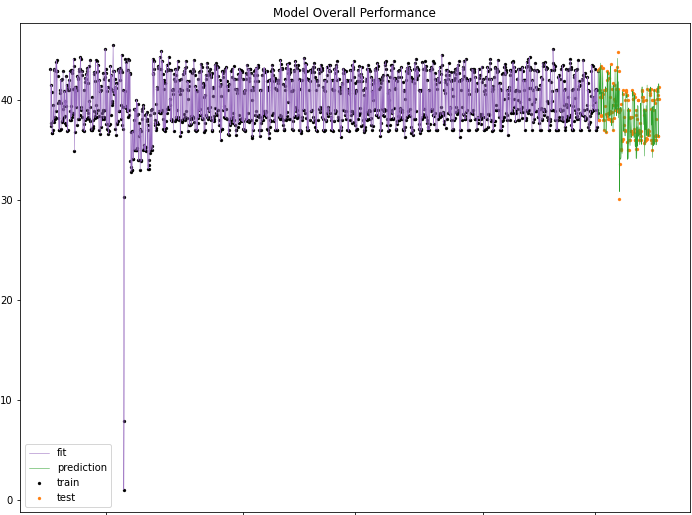
\includegraphics[width=0.6\linewidth]{xgb_reg_overall}
%	\caption{XGBoost overall performance}
%	\label{fig:xgb_reg_overall}
%\end{figure}
%
%\subsubsection*{Training fitting}
%
%\begin{figure}[H]
%	\centering
%	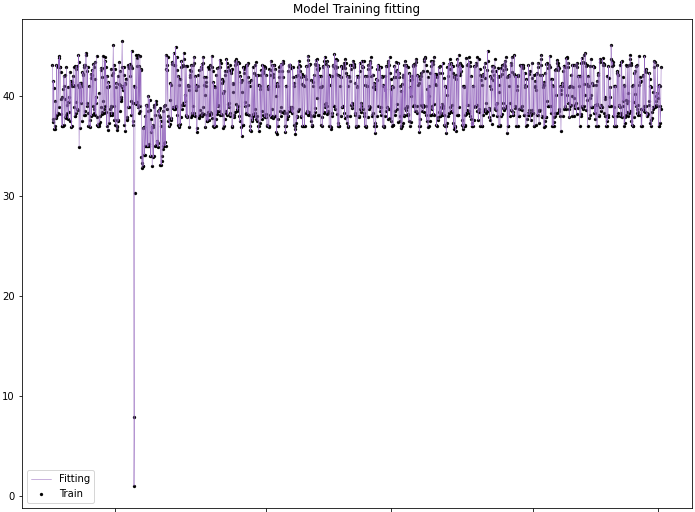
\includegraphics[width=0.6\linewidth]{xgb_reg_train}
%	\caption{XGBoost train performance}
%	\label{fig:xgb_reg_train}
%\end{figure}
%
%\begin{table}[H]
%	\centering
%	\begin{tabular}{|c|c|}
%		\hline
%		\ac{mae} 	& 0.04 \\
%		$R^2$ 		& 1.00 \\
%		\hline
%	\end{tabular}
%	\caption{XGBoost regressor train scores}
%	\label{table:xgb_reg_train_scores}
%\end{table}
%
%\subsubsection*{Test predictions}
%
%\begin{figure}[H]
%	\centering
%	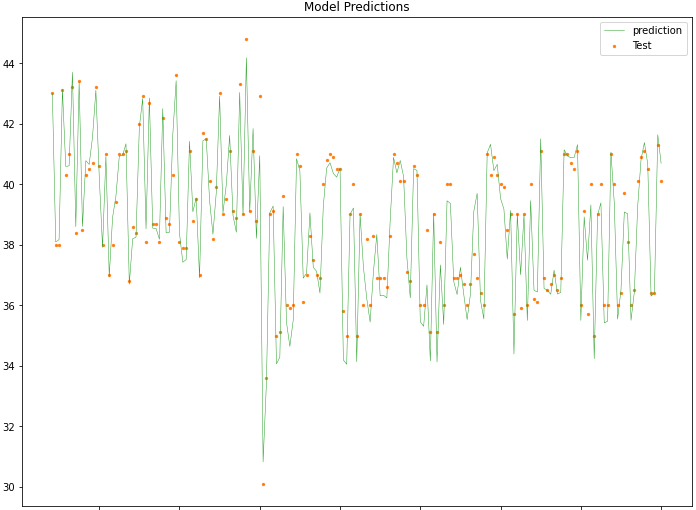
\includegraphics[width=0.6\linewidth]{xgb_reg_test}
%	\caption{XGBoost test performance}
%	\label{fig:xgb_reg_test}
%\end{figure}
%
%\begin{table}[H]
%	\centering
%	\begin{tabular}{|c|c|}
%		\hline
%		\ac{mae} 	& 0.44 \\
%		$R^2$ 		& 0.93 \\
%		\hline
%	\end{tabular}
%	\caption{XGBoost regressor prediction performance}
%	\label{table:xgb_reg_test_scores}
%\end{table}
%
%
%\subsubsection*{Residual analysis}
%
%\begin{figure}[hptb]
%	\begin{subfigure}{.47\textwidth}
%		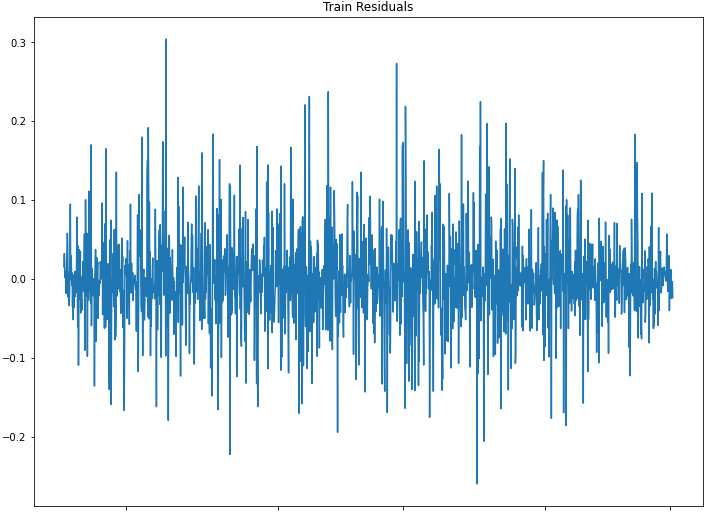
\includegraphics[width=\textwidth]{xgb_reg_res_train}
%		\caption{Train}
%		\label{fig:xgb_reg_res_train}
%	\end{subfigure}%
%	\hfill
%	\begin{subfigure}{.47\textwidth}
%		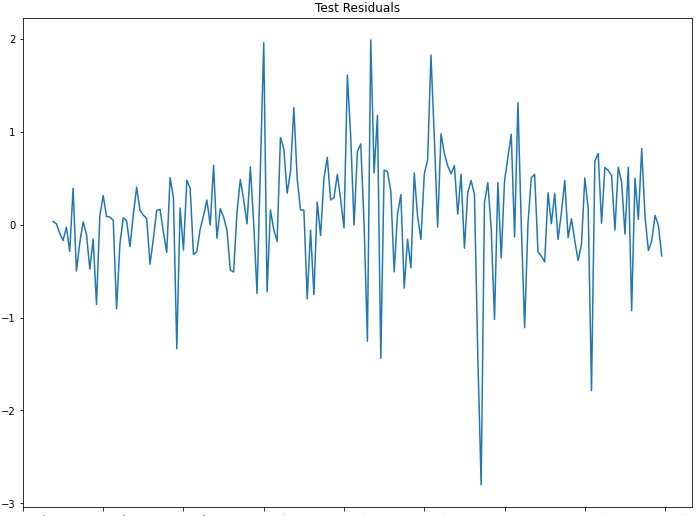
\includegraphics[width=\textwidth]{xgb_reg_res_test}
%		\caption{Test}
%		\label{fig:xgb_reg_res_test}
%	\end{subfigure}
%	\caption{XGBoost regression residuals}
%	\label{fig:xgb_reg_res}
%\end{figure}
%
%\begin{figure}[hptb]
%	\begin{subfigure}{.47\textwidth}
%		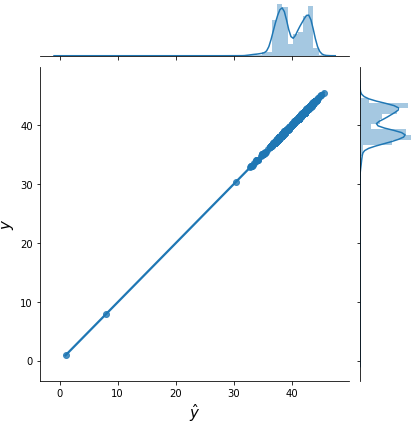
\includegraphics[width=\textwidth]{xgb_reg_joint_train}
%		\caption{Train}
%		\label{fig:xgb_reg_joint_train}
%	\end{subfigure}%
%	\hfill
%	\begin{subfigure}{.47\textwidth}
%		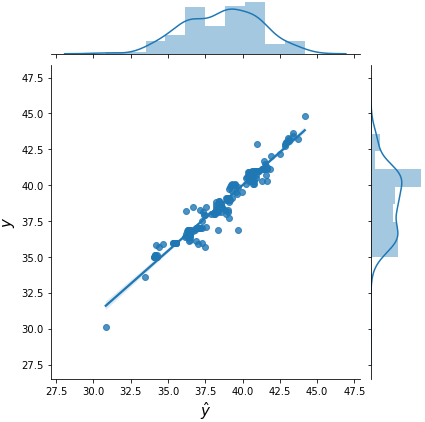
\includegraphics[width=\textwidth]{xgb_reg_joint_test}
%		\caption{Test}
%		\label{fig:xgb_reg_joint_test}
%	\end{subfigure}
%	\caption{XGBoost regression joint distributions of $y$ and $\hat{y}$}
%	\label{fig:xgb_reg_joint}
%\end{figure}
%
%\pagebreak
%\subsection{Including autoregressive components}
%
%Nonetheless, the function \ref{xgb_reg}, despite being trained to predict the next $y$ sample, still having only a regressive nature, i.e., no autoregressive components have been used to also learn from previous outputs. Thus, the function can be extended to:
%
%\begin{equation}
%	\label{xgb_ar}
%	y_{t} = \sum_{i=1}^{N}{\beta_i \cdot x_{{t-1}_i}} + \sum_{l=1}^{L}{\phi_l \cdot y_{t-l}}
%\end{equation}  
%
%Where $N$ is the amount of features and  $L$ corresponds to the amount of lags under consideration.
%
%\subsubsection*{Provisional results}
%
%\noindent\fbox{
%	\parbox{\textwidth}
%	{
%		Draft acknowledgement:\\
%		This section has a bug, which fixing will be resumed as soon as the report draft is delivered
%	}
%}
%
%\begin{figure}[H]
%	\centering
%	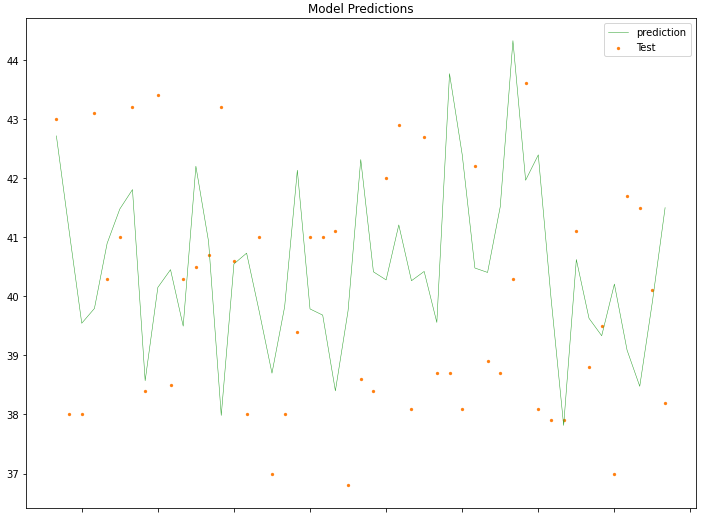
\includegraphics[width=0.6\linewidth]{xgb_ar_test}
%	\caption{XGBoost with autoregressive components test performance}
%	\label{fig:xgb_ar_test}
%\end{figure}
%
%\begin{figure}[hptb]
%	\begin{subfigure}{.47\textwidth}
%		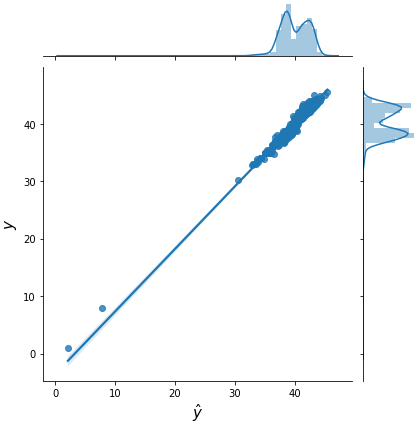
\includegraphics[width=\textwidth]{xgb_ar_joint_train}
%		\caption{Train}
%		\label{fig:xgb_ar_joint_train}
%	\end{subfigure}%
%	\hfill
%	\begin{subfigure}{.47\textwidth}
%		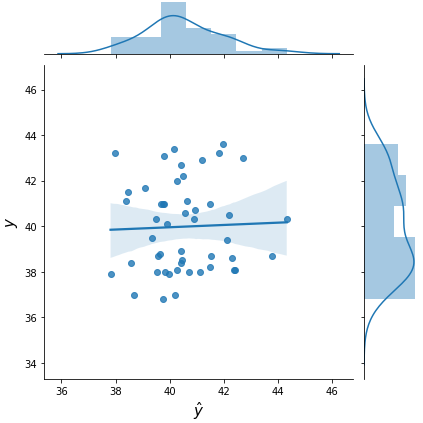
\includegraphics[width=\textwidth]{xgb_ar_joint_test}
%		\caption{Test}
%		\label{fig:xgb_ar_joint_test}
%	\end{subfigure}
%	\caption{XGBoost with autoregressive components joint distributions of $y$ and $\hat{y}$}
%	\label{fig:xgb_ar_joint}
%\end{figure}
